%!TEX program = xelatex
\documentclass[11pt,a4paper]{article}
\usepackage[utf8]{inputenc}
\usepackage[T1]{fontenc}
\usepackage{authblk}
\usepackage{ctex}
\usepackage{tikz}
\usepackage{pgfplots}
\usepackage{verbatim}
\usepackage{amsfonts}
\usepackage{amsmath}
\usepackage{amsthm}
\usepackage{indentfirst}
\usepackage{amssymb}
\usepackage{enumerate}
\setlength{\parindent}{0pt}
\usetikzlibrary{shapes,snakes}
\newcommand{\argmax}{\operatornamewithlimits{argmax}}
\newcommand{\argmin}{\operatornamewithlimits{argmin}}
\DeclareMathOperator{\col}{col}
\usepackage{booktabs}
\newtheorem{theorem}{Theorem}
\newtheorem{note}{Note}
\newtheorem{definition}{Definition}
\newtheorem{proposition}{Proposition}
\newtheorem{lemma}{Lemma}
\newtheorem{example}{Example}
\newtheorem{corollary}{Corollary}
\usepackage{graphicx}
\usepackage{geometry}
\usepackage{hyperref}
\newcommand{\code}{	exttt}
\geometry{a4paper,scale=0.8}
\title{Probability}
\author[*]{Wenxiao Yang}
\affil[*]{Department of Mathematics, University of Illinois at Urbana-Champaign}
\date{2021}


\begin{document}
\maketitle
\tableofcontents
\newpage


\section{Poisson Distribution $Pois(\lambda)$: 单位时间发生$k$次事件的概率}
\subsection{$\lambda$:单位时间发生该时间的平均次数}
$$\Pr(X{=}k)= \frac{\lambda^k e^{-\lambda}}{k!},\ k=0,1,2,3...$$
\subsection{$E(X)=Var(X)=\lambda$}
\subsection{推导}
我们考虑一段时间(讲单位时间微分成n等分, $n \rightarrow \infty$),每一刻(瞬间)都有一个event may occur, which follows binomial distribution $B(n,p)$. where $n \rightarrow \infty, p \rightarrow 0$; $\lambda=n\cdot p$ is the expected number of events in this period of time.\\
现在我们考虑发生$k$次event的概率:
\begin{equation}
    \begin{aligned}
        \Pr(X=k)&=\lim_{n \rightarrow\infty} \binom{n}{k} (\frac{\lambda}{n})^k(1-\frac{\lambda}{n})^{n-k}\\
        &=\lim_{n \rightarrow\infty} \frac{n!}{(n-k)!k!} (\frac{\lambda}{n})^k(1-\frac{\lambda}{n})^{n}(1-\frac{\lambda}{n})^{-k}\\
        &=\lim_{n \rightarrow\infty}\frac{n!}{(n-k)!k!} (\frac{\lambda}{n})^k e^{-\lambda}\\
        &=\frac{\lambda^k e^{-\lambda}}{k!}\lim_{n \rightarrow\infty}\frac{n!}{(n-k)!n^k}\\
        &=\frac{\lambda^k e^{-\lambda}}{k!}\lim_{n \rightarrow\infty}
        \frac{n}{n}\frac{n-1}{n}\cdots \frac{n-k+1}{n}\\
        &=\frac{\lambda^k e^{-\lambda}}{k!}
    \end{aligned}
    \nonumber
\end{equation}




\section{Exponential distribution $Exp(\lambda)$: 独立随机事件的发生间隔/第一次发生事件的时间}
\subsection{$\lambda$:单位时间发生该时间的平均次数}
随机变量$X$服从参数为$\lambda$ 或$\beta$ 的指数分布,则记作
$${\displaystyle X\sim {\text{Exp}}(\lambda )} \text{ or } {\displaystyle X\sim {\text{Exp}}(\beta )}$$
两者意义相同,只是$\lambda$ 与$\beta$ 互为倒数关系.
$${f(x;{\lambda})=\left\{{\begin{matrix}{\lambda }e^{-{\lambda }x}&x\geq 0\\0&\;x<0.\end{matrix}}\right.}$$
$${f(x;{\beta})=\left\{{\begin{matrix}{\frac{1}{\beta} }e^{-{\frac{1}{\beta} }x}&x\geq 0\\0&\;x<0.\end{matrix}}\right.}$$
累积分布函数为:
$${F(x;{\lambda})=\left\{{\begin{matrix}{1-}e^{-{\lambda }x}&x\geq 0\\0&\;x<0.\end{matrix}}\right.}$$
其中$\lambda > 0$是分布的参数,即每单位时间发生该事件的次数; $\beta>0$ 为尺度参数,即该事件在每单位时间内的发生率。两者常被称为率参数(rate parameter)。指数分布的区间是$[0,\infty)$。

\subsection{$\mathbb{E}(X)=\frac{1}{\lambda}$:预期事件的发生间隔; $Var(X)=\frac{1}{\lambda^2}$}
$$\mathbb{E}(X)=\frac{1}{\lambda};\ Var(X)=\frac{1}{\lambda^2}$$
\subsection{Memorylessness: ${\displaystyle \Pr \left(T>s+t\mid T>s\right)=\Pr(T>t)}$}
\begin{equation}
    \begin{aligned}
        \Pr (T>s+t\mid T>s)&=\frac{\Pr(T>s+t\text{ and }T>s)}{\Pr(T>s)}\\
        &=\frac{\Pr(T>s+t)}{\Pr(T>s)}\\
        &=\frac{e^{-\lambda(s+t)}}{e^{-\lambda s}}\\
        &=e^{-\lambda t}\\
        &=\Pr (T>t)
    \end{aligned}
    \nonumber
\end{equation}

\subsection{推导}
我们考虑一段时间(讲单位时间微分成n等分, $n \rightarrow \infty$),每一刻(瞬间)都有一个event may occur, which follows binomial distribution $B(n,p)$. where $n \rightarrow \infty, p \rightarrow 0$; $\lambda=n\cdot p$ is the expected number of events in this period of time. (与Poisson设定相同)\\
CDF: 现在我们考虑第一次发生event的时间大于x的概率:
\begin{equation}
    \begin{aligned}
        1-F(x;\lambda)=\lim_{n \rightarrow \infty}(1-\frac{\lambda}{n})^{nx}=e^{-\lambda x}
        \Rightarrow F(x;\lambda)=1-e^{-\lambda x}
    \end{aligned}
    \nonumber
\end{equation}
PDF:
\begin{equation}
    \begin{aligned}
        f(x;\lambda)=\frac{\partial F(x;\lambda)}{\partial x}=\lambda e^{-\lambda x}
    \end{aligned}
    \nonumber
\end{equation}

\section{Poisson process: A sequence of arrivals in continuous time with rate $\lambda$}
\subsection{Definition}
\subsubsection{$N(t)\sim Pois(\lambda t)$:Number of arrivals in length $t$ follows Poisson distribution}
\begin{equation}
    \begin{aligned}
        N(t)\sim Pois(\lambda t)\\
        \Pr(N(t)=k)=\frac{(\lambda t)^k e^{-\lambda t}}{k!}
    \end{aligned}
    \nonumber
\end{equation}
\subsubsection{The number of arrivals in disjoint time invervals are independent}
\subsection{$T_j$: time of $j^{th}$ arrival}
$T_1>t$ is same as $N(t)=0$: $P(T_1>t)=P(N(t)=0)=e^{-\lambda t}$\\
$\Rightarrow T_1\sim Expo(\lambda) \Rightarrow T_j-T_{j-1}\sim Expo(\lambda); T_j\sim Gamma(j,\lambda)$

\subsection{Theorem (Conditional counts): $N(t_1)|N(t_2)=n\sim Bin(n,\frac{t_1}{t_2})$}
可以理解为n个点散落在$(0,t_2]$上的概率每处均等$=\frac{1}{t_2}$; 所以散落在$(0,t_1]$上的概率为$\frac{t_1}{t_2}$

\section{Limit Theorems}
\subsection{Law of Large Numbers (LLN)}
Describe the behavior of the sample mean of i.i.d. as the sample size grows.

$x_{1}, x_{2}, \ldots, x_{n}$ i.i.d. with some distribution. $\mu<\infty,\sigma^{2}<\infty$,$\bar{x}=\frac{1}{n}\left(x_{1}+x_{2}+\cdots+x_{n}\right)$.

\begin{theorem}[Weak Law of Large Numbers (wLLN)]
    \quad

    The weak law of large numbers (also called Khinchin's law) states that the sample average \underline{converges in probability} towards the expected value.
    $${\displaystyle {\begin{matrix}{}\\{\overline {X}}_{n}\ {\xrightarrow {P}}\ \mu \qquad {\text{when}}\ n\to \infty .\\{}\end{matrix}}}$$
    That is, for any positive number $\varepsilon$,
    $${\displaystyle \lim _{n\to \infty }\Pr \!\left(\,|{\overline {X}}_{n}-\mu |<\varepsilon \,\right)=1.}$$
\end{theorem}
\begin{proof}
\quad

Proof: by Chebychev's inequality.
$$
\begin{aligned}
&P(|\bar{x}-\mu|\geq\varepsilon) \leq \frac{\sigma^{2}}{n \varepsilon^{2}} \quad (Var\bar{x}=\frac{\sigma^{2}}{n}) \\
&\lim_{n \rightarrow \infty}\frac{\sigma^{2}}{n \varepsilon^{2}}=0\\
\Rightarrow&\lim_{n \rightarrow \infty}P(|\bar{x}-\mu|>\varepsilon) \text { also converges to } 0 .
\end{aligned}
$$
\end{proof}

\begin{theorem}[Strong Law of Large Numbers (sLLN)]
    \quad

    With probability 1 (wp1) or almost surely (as).
    $${\displaystyle {\begin{matrix}{}\\{\overline {X}}_{n}\ {\xrightarrow {a.s.}}\ \mu \qquad {\text{when}}\ n\to \infty .\\{}\end{matrix}}}$$

    That is,
    $$\Pr \!\left(\lim _{n\to \infty }{\overline {X}}_{n}=\mu \right)=1.$$
\end{theorem}

\subsection{Differences between \underline{convergence in probability} (wLLN) and \underline{wp1(a.s.)} (sLLN)}
\begin{enumerate}[a)]
    \item Weak Law of Large Numbers (wLLN)
    $$P(|\bar{x}-\mu|\geq\varepsilon)\rightarrow 0\text{ as }n \rightarrow	+\infty,\ \forall \varepsilon>0$$
    \begin{center}\begin{figure}[htbp]
        \centering
        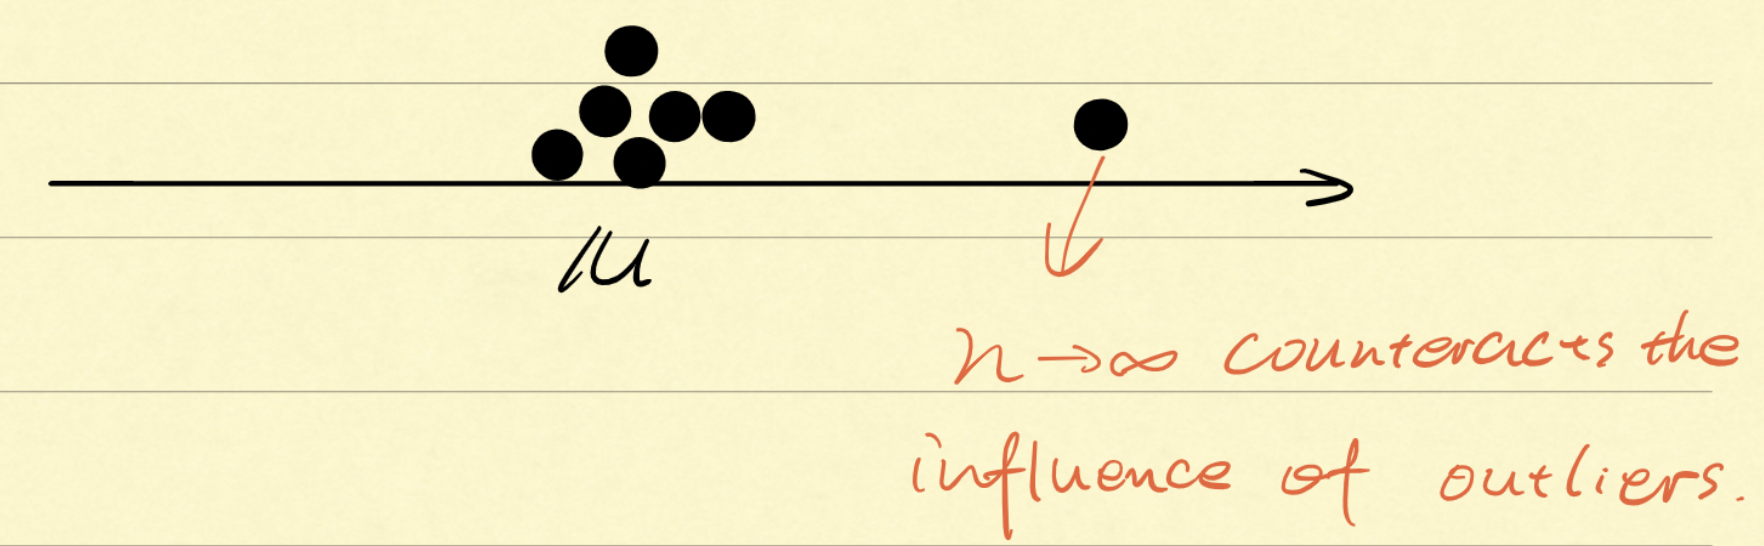
\includegraphics[scale=0.3]{wLLN.png}
        \caption{convergence in probability}
        \label{}
    \end{figure}\end{center}
    \item Strong Law of Large Numbers (sLLN)
    $$P(|\bar{x}-\mu|\geq\varepsilon\text{ as }n \rightarrow+\infty)=0,\ \forall \varepsilon>0$$
    \begin{center}\begin{figure}[htbp]
        \centering
        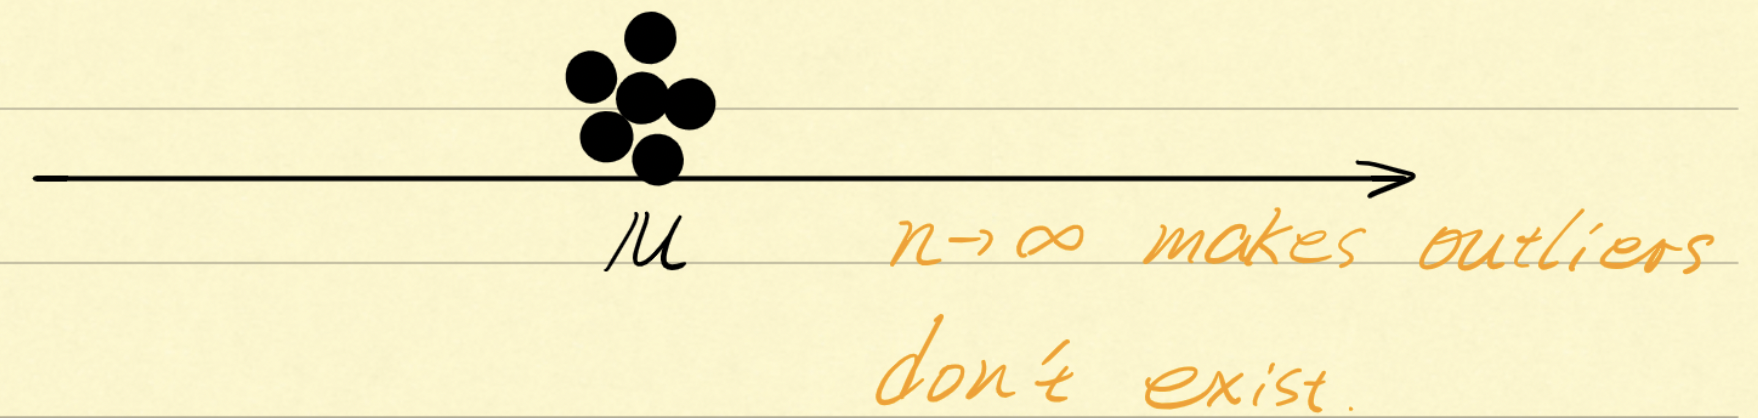
\includegraphics[scale=0.3]{sLLN.png}
        \caption{wp1(a.s.)}
        \label{}
    \end{figure}\end{center}
\end{enumerate}

\subsection{Central Limit Theorem (CLT)}
\begin{theorem}[Central Limit Theorem (CLT)]
    $$Z=\frac{\overline{X}-\mu}{\frac{\sigma}{\sqrt{n}}} \xrightarrow {D} N(0,1) \text{ when}\ n\to \infty$$
    $Z$ \underline{converges in distribution} to $N(0,1)$ as $n\to \infty$

    (converges in distribution: $P(\frac{\overline{X}-\mu}{\frac{\sigma}{\sqrt{n}}}\leq a)\rightarrow \frac{1}{\sqrt{2\pi}}\int_{-\infty}^ae^{-\frac{x^2}{2}}dx$)
\end{theorem}
\begin{proof}
    Prove the situation of $\mu=0,\sigma^2=1$, we can use linear transformations to get other situations.

    Moment-generating function(MGF) of $X_i$: $M_0(t)=E(e^{tX_i})$. $$M_0(0)=1,M_0'(0)=EX_i=0,M_0''(0)=EX_i^2=1$$
    Moment-generating function(MGF) of $\sqrt{n}\overline{X}$:
    \begin{equation}
        \begin{aligned}
            M_1(t)&=Ee^{t\sqrt{n}\overline{X}}=Ee^{t\frac{\sum_{i=1}^nX_i}{\sqrt{n}}\\
            %&=Ee^{t\frac{X_1}{\sqrt{n}}%\cdot Ee^{t\frac{X_2}{\sqrt{n}%})\cdots E(e^{t\frac{X_n}%{\sqrt{n}}\\
            %&=[M_0(\frac{t}{\sqrt{n}})]^n
        \end{aligned}
        \nonumber
    \end{equation}
\end{proof}






























\end{document}